\documentclass{ximera}

%\usepackage{todonotes}

\newcommand{\todo}{}

\usepackage{esint} % for \oiint
\ifxake%%https://math.meta.stackexchange.com/questions/9973/how-do-you-render-a-closed-surface-double-integral
\renewcommand{\oiint}{{\large\bigcirc}\kern-1.56em\iint}
\fi


\graphicspath{
  {./}
  {ximeraTutorial/}
  {basicPhilosophy/}
  {functionsOfSeveralVariables/}
  {normalVectors/}
  {lagrangeMultipliers/}
  {vectorFields/}
  {greensTheorem/}
  {shapeOfThingsToCome/}
  {dotProducts/}
  {partialDerivativesAndTheGradientVector/}
  {../productAndQuotientRules/exercises/}
  {../normalVectors/exercisesParametricPlots/}
  {../continuityOfFunctionsOfSeveralVariables/exercises/}
  {../partialDerivativesAndTheGradientVector/exercises/}
  {../directionalDerivativeAndChainRule/exercises/}
  {../commonCoordinates/exercisesCylindricalCoordinates/}
  {../commonCoordinates/exercisesSphericalCoordinates/}
  {../greensTheorem/exercisesCurlAndLineIntegrals/}
  {../greensTheorem/exercisesDivergenceAndLineIntegrals/}
  {../shapeOfThingsToCome/exercisesDivergenceTheorem/}
  {../greensTheorem/}
  {../shapeOfThingsToCome/}
  {../separableDifferentialEquations/exercises/}
  {vectorFields/}
}

\newcommand{\mooculus}{\textsf{\textbf{MOOC}\textnormal{\textsf{ULUS}}}}

\usepackage{tkz-euclide}
\usepackage{tikz}
\usepackage{tikz-cd}
\usetikzlibrary{arrows}
\tikzset{>=stealth,commutative diagrams/.cd,
  arrow style=tikz,diagrams={>=stealth}} %% cool arrow head
\tikzset{shorten <>/.style={ shorten >=#1, shorten <=#1 } } %% allows shorter vectors

\usetikzlibrary{backgrounds} %% for boxes around graphs
\usetikzlibrary{shapes,positioning}  %% Clouds and stars
\usetikzlibrary{matrix} %% for matrix
\usepgfplotslibrary{polar} %% for polar plots
\usepgfplotslibrary{fillbetween} %% to shade area between curves in TikZ
%\usetkzobj{all}
\usepackage[makeroom]{cancel} %% for strike outs
%\usepackage{mathtools} %% for pretty underbrace % Breaks Ximera
%\usepackage{multicol}
\usepackage{pgffor} %% required for integral for loops



%% http://tex.stackexchange.com/questions/66490/drawing-a-tikz-arc-specifying-the-center
%% Draws beach ball
\tikzset{pics/carc/.style args={#1:#2:#3}{code={\draw[pic actions] (#1:#3) arc(#1:#2:#3);}}}



\usepackage{array}
\setlength{\extrarowheight}{+.1cm}
\newdimen\digitwidth
\settowidth\digitwidth{9}
\def\divrule#1#2{
\noalign{\moveright#1\digitwidth
\vbox{\hrule width#2\digitwidth}}}




% \newcommand{\RR}{\mathbb R}
% \newcommand{\R}{\mathbb R}
% \newcommand{\N}{\mathbb N}
% \newcommand{\Z}{\mathbb Z}

\newcommand{\sagemath}{\textsf{SageMath}}


%\renewcommand{\d}{\,d\!}
%\renewcommand{\d}{\mathop{}\!d}
%\newcommand{\dd}[2][]{\frac{\d #1}{\d #2}}
%\newcommand{\pp}[2][]{\frac{\partial #1}{\partial #2}}
% \renewcommand{\l}{\ell}
%\newcommand{\ddx}{\frac{d}{\d x}}

% \newcommand{\zeroOverZero}{\ensuremath{\boldsymbol{\tfrac{0}{0}}}}
%\newcommand{\inftyOverInfty}{\ensuremath{\boldsymbol{\tfrac{\infty}{\infty}}}}
%\newcommand{\zeroOverInfty}{\ensuremath{\boldsymbol{\tfrac{0}{\infty}}}}
%\newcommand{\zeroTimesInfty}{\ensuremath{\small\boldsymbol{0\cdot \infty}}}
%\newcommand{\inftyMinusInfty}{\ensuremath{\small\boldsymbol{\infty - \infty}}}
%\newcommand{\oneToInfty}{\ensuremath{\boldsymbol{1^\infty}}}
%\newcommand{\zeroToZero}{\ensuremath{\boldsymbol{0^0}}}
%\newcommand{\inftyToZero}{\ensuremath{\boldsymbol{\infty^0}}}



% \newcommand{\numOverZero}{\ensuremath{\boldsymbol{\tfrac{\#}{0}}}}
% \newcommand{\dfn}{\textbf}
% \newcommand{\unit}{\,\mathrm}
% \newcommand{\unit}{\mathop{}\!\mathrm}
% \newcommand{\eval}[1]{\bigg[ #1 \bigg]}
% \newcommand{\seq}[1]{\left( #1 \right)}
% \renewcommand{\epsilon}{\varepsilon}
% \renewcommand{\phi}{\varphi}


% \renewcommand{\iff}{\Leftrightarrow}

% \DeclareMathOperator{\arccot}{arccot}
% \DeclareMathOperator{\arcsec}{arcsec}
% \DeclareMathOperator{\arccsc}{arccsc}
% \DeclareMathOperator{\si}{Si}
% \DeclareMathOperator{\scal}{scal}
% \DeclareMathOperator{\sign}{sign}


%% \newcommand{\tightoverset}[2]{% for arrow vec
%%   \mathop{#2}\limits^{\vbox to -.5ex{\kern-0.75ex\hbox{$#1$}\vss}}}
% \newcommand{\arrowvec}[1]{{\overset{\rightharpoonup}{#1}}}
% \renewcommand{\vec}[1]{\arrowvec{\mathbf{#1}}}
% \renewcommand{\vec}[1]{{\overset{\boldsymbol{\rightharpoonup}}{\mathbf{#1}}}}

% \newcommand{\point}[1]{\left(#1\right)} %this allows \vector{ to be changed to \vector{ with a quick find and replace
% \newcommand{\pt}[1]{\mathbf{#1}} %this allows \vec{ to be changed to \vec{ with a quick find and replace
% \newcommand{\Lim}[2]{\lim_{\point{#1} \to \point{#2}}} %Bart, I changed this to point since I want to use it.  It runs through both of the exercise and exerciseE files in limits section, which is why it was in each document to start with.

% \DeclareMathOperator{\proj}{\mathbf{proj}}
% \newcommand{\veci}{{\boldsymbol{\hat{\imath}}}}
% \newcommand{\vecj}{{\boldsymbol{\hat{\jmath}}}}
% \newcommand{\veck}{{\boldsymbol{\hat{k}}}}
% \newcommand{\vecl}{\vec{\boldsymbol{\l}}}
% \newcommand{\uvec}[1]{\mathbf{\hat{#1}}}
% \newcommand{\utan}{\mathbf{\hat{t}}}
% \newcommand{\unormal}{\mathbf{\hat{n}}}
% \newcommand{\ubinormal}{\mathbf{\hat{b}}}

% \newcommand{\dotp}{\bullet}
% \newcommand{\cross}{\boldsymbol\times}
% \newcommand{\grad}{\boldsymbol\nabla}
% \newcommand{\divergence}{\grad\dotp}
% \newcommand{\curl}{\grad\cross}
%\DeclareMathOperator{\divergence}{divergence}
%\DeclareMathOperator{\curl}[1]{\grad\cross #1}
% \newcommand{\lto}{\mathop{\longrightarrow\,}\limits}

% \renewcommand{\bar}{\overline}

\colorlet{textColor}{black}
\colorlet{background}{white}
\colorlet{penColor}{blue!50!black} % Color of a curve in a plot
\colorlet{penColor2}{red!50!black}% Color of a curve in a plot
\colorlet{penColor3}{red!50!blue} % Color of a curve in a plot
\colorlet{penColor4}{green!50!black} % Color of a curve in a plot
\colorlet{penColor5}{orange!80!black} % Color of a curve in a plot
\colorlet{penColor6}{yellow!70!black} % Color of a curve in a plot
\colorlet{fill1}{penColor!20} % Color of fill in a plot
\colorlet{fill2}{penColor2!20} % Color of fill in a plot
\colorlet{fillp}{fill1} % Color of positive area
\colorlet{filln}{penColor2!20} % Color of negative area
\colorlet{fill3}{penColor3!20} % Fill
\colorlet{fill4}{penColor4!20} % Fill
\colorlet{fill5}{penColor5!20} % Fill
\colorlet{gridColor}{gray!50} % Color of grid in a plot

\newcommand{\surfaceColor}{violet}
\newcommand{\surfaceColorTwo}{redyellow}
\newcommand{\sliceColor}{greenyellow}




\pgfmathdeclarefunction{gauss}{2}{% gives gaussian
  \pgfmathparse{1/(#2*sqrt(2*pi))*exp(-((x-#1)^2)/(2*#2^2))}%
}


%%%%%%%%%%%%%
%% Vectors
%%%%%%%%%%%%%

%% Simple horiz vectors
\renewcommand{\vector}[1]{\left\langle #1\right\rangle}


%% %% Complex Horiz Vectors with angle brackets
%% \makeatletter
%% \renewcommand{\vector}[2][ , ]{\left\langle%
%%   \def\nextitem{\def\nextitem{#1}}%
%%   \@for \el:=#2\do{\nextitem\el}\right\rangle%
%% }
%% \makeatother

%% %% Vertical Vectors
%% \def\vector#1{\begin{bmatrix}\vecListA#1,,\end{bmatrix}}
%% \def\vecListA#1,{\if,#1,\else #1\cr \expandafter \vecListA \fi}

%%%%%%%%%%%%%
%% End of vectors
%%%%%%%%%%%%%

%\newcommand{\fullwidth}{}
%\newcommand{\normalwidth}{}



%% makes a snazzy t-chart for evaluating functions
%\newenvironment{tchart}{\rowcolors{2}{}{background!90!textColor}\array}{\endarray}

%%This is to help with formatting on future title pages.
\newenvironment{sectionOutcomes}{}{}



%% Flowchart stuff
%\tikzstyle{startstop} = [rectangle, rounded corners, minimum width=3cm, minimum height=1cm,text centered, draw=black]
%\tikzstyle{question} = [rectangle, minimum width=3cm, minimum height=1cm, text centered, draw=black]
%\tikzstyle{decision} = [trapezium, trapezium left angle=70, trapezium right angle=110, minimum width=3cm, minimum height=1cm, text centered, draw=black]
%\tikzstyle{question} = [rectangle, rounded corners, minimum width=3cm, minimum height=1cm,text centered, draw=black]
%\tikzstyle{process} = [rectangle, minimum width=3cm, minimum height=1cm, text centered, draw=black]
%\tikzstyle{decision} = [trapezium, trapezium left angle=70, trapezium right angle=110, minimum width=3cm, minimum height=1cm, text centered, draw=black]


\title{The Key}

\begin{document}

\begin{abstract}
circles and triangles
\end{abstract}
\maketitle





\textbf{\textcolor{red!70!black}{All}}, \textbf{\textcolor{red!80!black}{Every}}, \textbf{\textcolor{red!80!black}{None}} - These are the words of mathematics. 



\begin{itemize}
\item The position of \textbf{\textcolor{red!70!black}{every}} point in the Cartesian plane can be described as a scalar times a direction vector.  

\item \textbf{\textcolor{red!70!black}{Every}} Complex number can be represented as the product of a real number and a complex number with modulus $1$.

\item \textbf{\textcolor{red!70!black}{Every}} Complex number can be represented as the product of a real number and a complex number that sits on the unit circle.

\item \textbf{\textcolor{red!70!black}{Every}} Complex number can be represented in the form \textbf{\textcolor{purple!85!blue}{$r \cdot (\cos(\theta) + i \, \sin(\theta))$}}.
\end{itemize}








\begin{image}
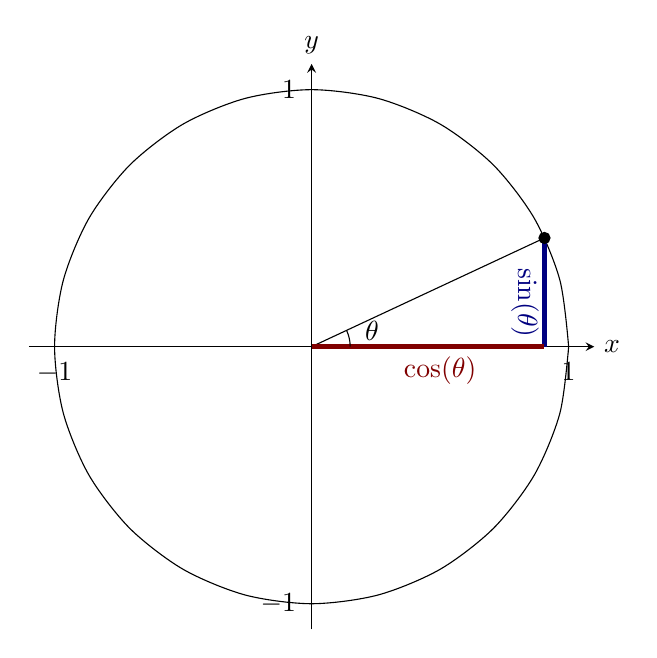
\begin{tikzpicture}
  \begin{axis}[
            xmin=-1.1,xmax=1.1,ymin=-1.1,ymax=1.1,
            axis lines=center,
            width=4in,
            xtick={-1,1},
            ytick={-1,1},
            clip=false,
            unit vector ratio*=1 1 1,
            xlabel=$x$, ylabel=$y$,
            every axis y label/.style={at=(current axis.above origin),anchor=south},
            every axis x label/.style={at=(current axis.right of origin),anchor=west},
          ]        

          

          \addplot [smooth, domain=(0:360)] ({cos(x)},{sin(x)}); %% unit circle

          \addplot [textColor] plot coordinates {(0,0) (0.906,0.423)}; %% 40 degrees

          \addplot [ultra thick,penColor] plot coordinates {(0.906,0) (0.906,0.423)}; %% 40 degrees
          \addplot [ultra thick,penColor2] plot coordinates {(0,0) (0.906,0)}; %% 40 degrees
          
          %\addplot [ultra thick,penColor3] plot coordinates {(1,0) (1,.839)}; %% 40 degrees          

          \addplot [textColor,smooth, domain=(0:25)] ({0.15*cos(x)},{0.15*sin(x)});
          %\addplot [very thick,penColor] plot coordinates {(0,0) (.766,.643)}; %% sector
          %\addplot [very thick,penColor] plot coordinates {(0,0) (1,0)}; %% sector
          %\addplot [very thick, penColor, smooth, domain=(0:40)] ({cos(x)},{sin(x)}); %% sector
          \node at (axis cs:0.17,0.06) [anchor=west] {$\theta$};
          \node[penColor, rotate=-90] at (axis cs:0.83,0.17) {$\sin(\theta)$};
          \node[penColor2] at (axis cs:0.5,0) [anchor=north] {$\cos(\theta)$};
          %\node[penColor3, rotate=-90] at (axis cs:1.06,.322) {$\tan(\theta)$};

          \addplot[color=black,fill=black,only marks,mark=*] coordinates{(0.906,0.423)};


        \end{axis}
\end{tikzpicture}
\end{image}



If we can understand the unit circle in terms of complex numbers, then we will have a good understanding of all complex numbers.






$\blacktriangleright$ \textbf{\textcolor{blue!75!black}{Multiplication on the Unit Circle}}  \\


Pretend we have two Complex numbers on the unit circle.

\begin{itemize}
\item $C_1 = a + b \, i$ with $|C_1| = 1$
\item $C_2 = c + d \, i$ with $|C_2| = 1$
\end{itemize}



We know $a^2 + b^2 = 1$  and $c^2 + d^2 = 1$.



Now, let's examine their product.






\begin{align*}
(a + b \, i) \cdot (c + d \, i)      & = ac + ad \, i + bc \, i - bd   \\
                & = (ac - bd) + (ad + bd) \, i
\end{align*}



What is the modulus of the product?





\begin{align*}
|(a + b \, i) \cdot (c + d \, i)|      & = | (ac - bd) + (ad + bd) \, i | \\
                & = (ac - bd)^2 + (ad + bd)^2   \\
                & = a^2c^2 - 2abcd + b^2d^2 + a^2d^2 + 2abcd + b^2c^2  \\
                & = a^2c^2 + b^2d^2 + a^2d^2 + b^2c^2  \\
                & = (a^2 + b^2) \cdot (c^2 + d^2)   \\
                & = 1 \cdot 1  \\
                & = 1
\end{align*}



\textbf{\textcolor{purple!85!blue}{The product is again on the unit circle!}}





\textbf{Question:} Where is this product on the unit circle?














\section*{Polar Perspective}



The complex number $C_1 = a + b \, i$, is positioned at an angle $\theta$ from the positive $x$-axis and a distance $r_1$ from the origin. Therefore, it has the polar form $(r_1, \theta)$. But if  $a + b \, i$ is on the unit circle, then $r_1 = 1$ and the polar form is $(1, \theta)$.




This point defines a right triangle with base $a$ and height $b$ and angle $\theta$ .  









\begin{image}
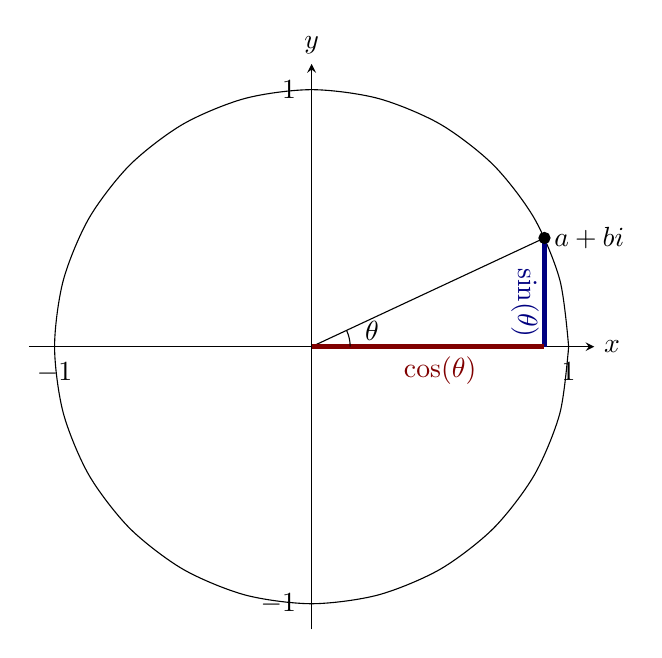
\begin{tikzpicture}
  \begin{axis}[
            xmin=-1.1,xmax=1.1,ymin=-1.1,ymax=1.1,
            axis lines=center,
            width=4in,
            xtick={-1,1},
            ytick={-1,1},
            clip=false,
            unit vector ratio*=1 1 1,
            xlabel=$x$, ylabel=$y$,
            every axis y label/.style={at=(current axis.above origin),anchor=south},
            every axis x label/.style={at=(current axis.right of origin),anchor=west},
          ]        

          \addplot [smooth, domain=(0:360)] ({cos(x)},{sin(x)}); %% unit circle

          \addplot [textColor] plot coordinates {(0,0) (0.906,0.423)}; %% 40 degrees

          \addplot [ultra thick,penColor] plot coordinates {(0.906,0) (0.906,0.423)}; %% 40 degrees
          \addplot [ultra thick,penColor2] plot coordinates {(0,0) (0.906,0)}; %% 40 degrees
          
          %\addplot [ultra thick,penColor3] plot coordinates {(1,0) (1,.839)}; %% 40 degrees          

          \addplot [textColor,smooth, domain=(0:25)] ({0.15*cos(x)},{0.15*sin(x)});
          %\addplot [very thick,penColor] plot coordinates {(0,0) (.766,.643)}; %% sector
          %\addplot [very thick,penColor] plot coordinates {(0,0) (1,0)}; %% sector
          %\addplot [very thick, penColor, smooth, domain=(0:40)] ({cos(x)},{sin(x)}); %% sector
          \node at (axis cs:0.17,0.06) [anchor=west] {$\theta$};
          \node[penColor, rotate=-90] at (axis cs:0.83,0.17) {$\sin(\theta)$};
          \node[penColor2] at (axis cs:0.5,0) [anchor=north] {$\cos(\theta)$};
          %\node[penColor3, rotate=-90] at (axis cs:1.06,.322) {$\tan(\theta)$};


          \node at (axis cs:0.906,0.423) [anchor=west] {$a + bi$};

          \addplot[color=black,fill=black,only marks,mark=*] coordinates{(0.906,0.423)};

        \end{axis}
\end{tikzpicture}
\end{image}





Above is a diagram of the right triangle for $a + b \, i = (1, \theta)$. \\




The complex number $C_2 = c + d \, i$, has a polar form $(r_2, \phi)$, which similarly is $(1, \phi)$.  Normally, we would plot a point for this complex number by rotating counterclockwise an angle $\phi$ from the positive $x$-axis.  Instead, we are going to tack on this angle to $\theta$.

So, we are sort of pretending that the radius for the first complex number, $a + b \, i$, is acting like a new $x$-axis and we are going to rotate counterclockwise an angle $\phi$ from that radius.





We begin making a right triangle for   $c + d \, i$ with an angle $\phi$.





\begin{image}[3in]
    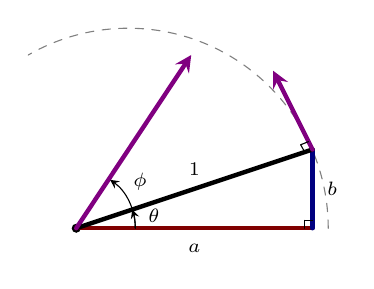
\begin{tikzpicture}[line cap=round]


  \draw [gray,thin,dashed] (3.2,0) arc (0:120:1in); 
  \draw [black,fill=black] (0,0) circle (0.05cm);

  %\draw [ultra thick] (0,0) -- (0,3);
  \draw [penColor2,ultra thick] (0,0) -- (3,0);
  \draw [penColor,ultra thick] (3,0) -- (3,1);
  %\draw [ultra thick,->] (1,0) -- (3,3);
  %\draw [ultra thick] (0,3) -- (3,3);

  \draw [ultra thick] (0,0) -- (3,1);
  \draw [penColor3,ultra thick,->] (3,1) -- (2.5,2);
  \draw [penColor3,ultra thick,->] (0,0) -- (1.46,2.2);

  \draw [thin] (2.9,0) -- (2.9,0.1);
  \draw [thin] (2.9,0.1) -- (3,0.1);

  \draw [thin] (2.9,0.97) -- (2.85,1.06);
  \draw [thin] (2.85,1.06) -- (2.95,1.10);


 

  \draw [->] (.75,0) arc(0:18.4:.75); 
  \draw [rotate=9] (1,0) node {\scriptsize{$\theta$}};
  \draw [->] (.75,0) arc(0:55:.75); 
  \draw [rotate=36] (1,0) node {\scriptsize{$\phi$}};


  \draw (1.5,-0.25) node {\scriptsize{$a$}};
  \draw (3.25,0.5) node {\scriptsize{$b$}};
  \draw (1.5,0.75) node {\scriptsize{$1$}};


  %\draw (2.9,1.5) node {\scriptsize{$\theta$}};






    \end{tikzpicture}
  \end{image}




Eventually, the sides meet to make a right triangle.  Let's enclose the whole diagram with a rectangle at that height.









\begin{image}[3in]
    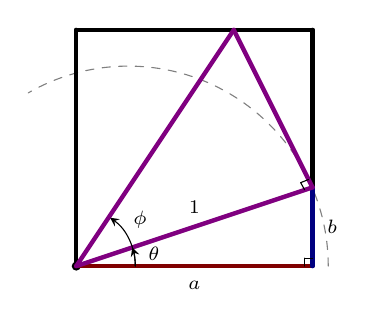
\begin{tikzpicture}[line cap=round]

  \draw [gray,thin,dashed] (3.2,0) arc (0:120:1in); 
  \draw [black,fill=black] (0,0) circle (0.05cm);

  \draw [ultra thick] (0,0) -- (0,3);
  \draw [penColor2,ultra thick] (0,0) -- (3,0);
  \draw [ultra thick] (3,1) -- (3,3);
  \draw [penColor,ultra thick] (3,0) -- (3,1);
  \draw [ultra thick] (0,3) -- (3,3);

  \draw [penColor3,ultra thick] (0,0) -- (3,1);
  \draw [penColor3,ultra thick] (3,1) -- (2,3);
  \draw [penColor3,ultra thick] (0,0) -- (2,3);

  \draw [thin] (2.9,0) -- (2.9,0.1);
  \draw [thin] (2.9,0.1) -- (3,0.1);

  \draw [thin] (2.9,0.97) -- (2.85,1.06);
  \draw [thin] (2.85,1.06) -- (2.95,1.10);




  \draw [->] (.75,0) arc(0:18.4:.75); 
  \draw [rotate=9] (1,0) node {\scriptsize{$\theta$}};
  \draw [->] (.75,0) arc(0:55:.75); 
  \draw [rotate=36] (1,0) node {\scriptsize{$\phi$}};


  \draw (1.5,-0.25) node {\scriptsize{$a$}};
  \draw (3.25,0.5) node {\scriptsize{$b$}};
  \draw (1.5,0.75) node {\scriptsize{$1$}};


  %\draw (2.9,1.5) node {\scriptsize{$\theta$}};






    \end{tikzpicture}
  \end{image}








The problem is that this second right triangle is too big for our unit circle. It is supposed to be a right triangle for $c + d \, i$.  That means the sides were suppose to be $c$ and $d$.  The hypotenuse was suppose to be of length $1$, to be a radius on the unit circle. Instead, in our diagram, the bottom leg has length $1$. That is too much.  That is ok. We can still get the lengths of this triangle.  

So, our new right triangle is not the $c-d-1$ right triangle for $c + d \, i$. \\


 The good news is that the new triangle we created is a right triangle with angle $\phi$.  That means it is similar to the $c-d-1$ right triangle for $c + d \, i$.  The sides must be proportional to the sides of the $c-d-1$ right triangle for $c + d \, i$.  We can use this proportionality.

  Let's call the lengths of the sides of this new trinagle $k$ and $h$.  $k$ is one of the legs of the right triangle and $h$ is the hypotenuse.










\begin{image}[3in]
    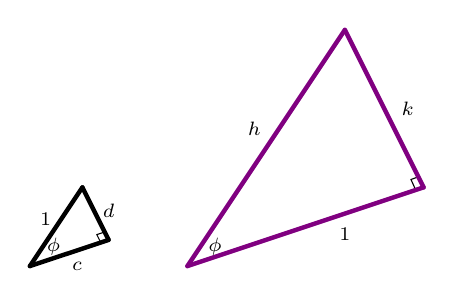
\begin{tikzpicture}[line cap=round]



  \draw [,thin] (2.9,0.966) -- (2.84,1.1);
  \draw [thin] (2.95,1.14) -- (2.84,1.1);


  \draw [thin] (-1.1,0.2997) -- (-1.15,0.3997);
  \draw [thin] (-1.15,0.3997) -- (-1.05,0.433);


  \draw [penColor3,ultra thick] (0,0) -- (3,1);
  \draw [penColor3,ultra thick] (3,1) -- (2,3);
  \draw [penColor3,ultra thick] (0,0) -- (2,3);

  \draw [rotate=0] (0.35,0.25) node {\scriptsize{$\phi$}};
  %\draw [rotate=0] (2.75,1.1) node {\scriptsize{$\beta$}};
  %\draw [rotate=0] (2,2.7) node {\scriptsize{$\phi$}};

  \draw (-1.4,0) node {\scriptsize{$c$}};
  \draw (-1,0.7) node {\scriptsize{$d$}};
  \draw (-1.8,0.6) node {\scriptsize{$1$}};





  \draw [ultra thick] (-2,0) -- (-1,0.333);
  \draw [ultra thick] (-1,0.333) -- (-1.333,1);
  \draw [ultra thick] (-2,0) -- (-1.333,1);

  \draw [rotate=0] (-1.7,0.25) node {\scriptsize{$\phi$}};
  %\draw [rotate=0] (-1.2,0.4) node {\scriptsize{$\beta$}};
  %\draw [rotate=0] (-1.35,0.75) node {\scriptsize{$\phi$}};

  \draw (2.8,2) node {\scriptsize{$k$}};
  \draw (0.85,1.75) node {\scriptsize{$h$}};
  \draw (2,0.4) node {\scriptsize{$1$}};


  %\draw [ultra thick,->] (-1.5,2) -- (0.5,2);
  %\draw [rotate=0] (-0.5,2.25) node {\scriptsize{factor of $k$}};










    \end{tikzpicture}
  \end{image}

These right triangles are similar.


\[
\frac{h}{1} = \frac{k}{d} = \frac{1}{c}
\]

\[
k = \frac{d}{c}
\]



The other leg of our right triangle has length $\frac{d}{c}$.










\begin{image}[3in]
    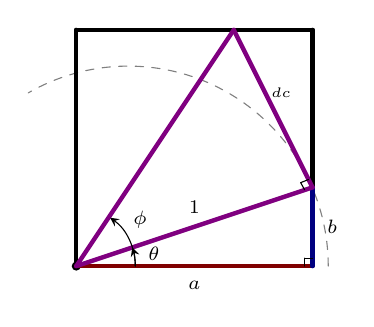
\begin{tikzpicture}[line cap=round]

  \draw [gray,thin,dashed] (3.2,0) arc (0:120:1in); 
  \draw [black,fill=black] (0,0) circle (0.05cm);

  \draw [ultra thick] (0,0) -- (0,3);
  \draw [penColor2,ultra thick] (0,0) -- (3,0);
  \draw [ultra thick] (3,1) -- (3,3);
  \draw [penColor,ultra thick] (3,0) -- (3,1);
  \draw [ultra thick] (0,3) -- (3,3);

  \draw [penColor3,ultra thick] (0,0) -- (3,1);
  \draw [penColor3,ultra thick] (3,1) -- (2,3);
  \draw [penColor3,ultra thick] (0,0) -- (2,3);

  \draw [thin] (2.9,0) -- (2.9,0.1);
  \draw [thin] (2.9,0.1) -- (3,0.1);

  \draw [thin] (2.9,0.97) -- (2.85,1.06);
  \draw [thin] (2.85,1.06) -- (2.95,1.10);




  \draw [->] (.75,0) arc(0:18.4:.75); 
  \draw [rotate=9] (1,0) node {\scriptsize{$\theta$}};
  \draw [->] (.75,0) arc(0:55:.75); 
  \draw [rotate=36] (1,0) node {\scriptsize{$\phi$}};


  \draw (1.5,-0.25) node {\scriptsize{$a$}};
  \draw (3.25,0.5) node {\scriptsize{$b$}};
  \draw (1.5,0.75) node {\scriptsize{$1$}};

  \draw (2.6,2.2) node {\tiny{$\tfrac{d}{c}$}};


  %\draw (2.9,1.5) node {\scriptsize{$\theta$}};






    \end{tikzpicture}
  \end{image}










We can also deduce some information about the top-right right triangle in this diagram. 


If we label the angles $\alpha$ and $\beta$ in the diagram below, then




\begin{itemize}
  \item Our original right triangle for $a + b \, i$  has non-right angles, $\theta$, and angle $\beta$.
  \item The right side of the big encompassing rectangle forms a straight angle and it is cut up into three angles: a right angle, $\beta$ on one side, and $\alpha$ on the other side. The sum must be $180^{\circ}$.
\end{itemize}















\begin{image}[3in]
    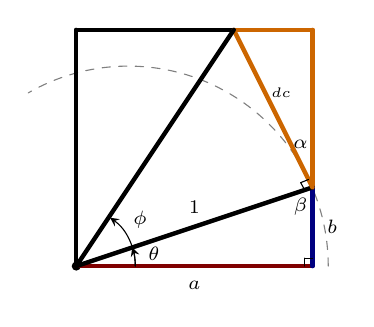
\begin{tikzpicture}[line cap=round]

  \draw [gray,thin,dashed] (3.2,0) arc (0:120:1in); 
  \draw [black,fill=black] (0,0) circle (0.05cm);

  \draw [ultra thick] (0,0) -- (0,3);
  \draw [penColor2,ultra thick] (0,0) -- (3,0);
  \draw [penColor5,ultra thick] (3,1) -- (3,3);
  \draw [penColor,ultra thick] (3,0) -- (3,1);
  \draw [ultra thick] (0,3) -- (2,3);
  \draw [penColor5,ultra thick] (2,3) -- (3,3);

  \draw [ultra thick] (0,0) -- (3,1);
  \draw [penColor5, ultra thick] (3,1) -- (2,3);
  \draw [ultra thick] (0,0) -- (2,3);

  \draw [thin] (2.9,0) -- (2.9,0.1);
  \draw [thin] (2.9,0.1) -- (3,0.1);

  \draw [thin] (2.9,0.97) -- (2.85,1.06);
  \draw [thin] (2.85,1.06) -- (2.95,1.10);




  \draw [->] (.75,0) arc(0:18.4:.75); 
  \draw [rotate=9] (1,0) node {\scriptsize{$\theta$}};
  \draw [->] (.75,0) arc(0:55:.75); 
  \draw [rotate=36] (1,0) node {\scriptsize{$\phi$}};


  \draw (1.5,-0.25) node {\scriptsize{$a$}};
  \draw (3.25,0.5) node {\scriptsize{$b$}};
  \draw (1.5,0.75) node {\scriptsize{$1$}};

  \draw (2.6,2.2) node {\tiny{$\tfrac{d}{c}$}};


  \draw (2.85,1.55) node {\scriptsize{$\alpha$}};
  \draw (2.85,0.75) node {\scriptsize{$\beta$}};






    \end{tikzpicture}
  \end{image}







The sum of the angles of the bottom right triangle is $\theta + \beta + 90^{\circ} = 180^{\circ}$ and the angles forming the straight angle sum to $\beta + \alpha + 90^{\circ} = 180^{\circ}$.  




\[
\theta + \beta + 90^{\circ}   =   \beta + \alpha + 90^{\circ}
\]



\[  \theta = \alpha  \]






The angles in the top-right right triangle are also $\theta$ and $\beta$. 


The bottom right triangle representing $a + b \, i$ and the triangle formed in the upper-right corner of the rectangle are similar triangles.  We can get the lengths of the legs of the top right triangle. Let's call these lengths $x$ and $y$ in the diagram.









\begin{image}[3in]
    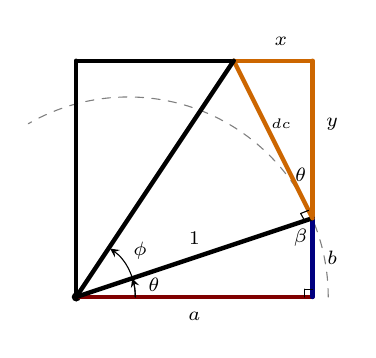
\begin{tikzpicture}[line cap=round]

  \draw [gray,thin,dashed] (3.2,0) arc (0:120:1in); 
  \draw [black,fill=black] (0,0) circle (0.05cm);

  \draw [ultra thick] (0,0) -- (0,3);
  \draw [penColor2,ultra thick] (0,0) -- (3,0);
  \draw [penColor5,ultra thick] (3,1) -- (3,3);
  \draw [penColor,ultra thick] (3,0) -- (3,1);
  \draw [ultra thick] (0,3) -- (2,3);
  \draw [penColor5,ultra thick] (2,3) -- (3,3);

  \draw [ultra thick] (0,0) -- (3,1);
  \draw [penColor5, ultra thick] (3,1) -- (2,3);
  \draw [ultra thick] (0,0) -- (2,3);

  \draw [thin] (2.9,0) -- (2.9,0.1);
  \draw [thin] (2.9,0.1) -- (3,0.1);

  \draw [thin] (2.9,0.97) -- (2.85,1.06);
  \draw [thin] (2.85,1.06) -- (2.95,1.10);




  \draw [->] (.75,0) arc(0:18.4:.75); 
  \draw [rotate=9] (1,0) node {\scriptsize{$\theta$}};
  \draw [->] (.75,0) arc(0:55:.75); 
  \draw [rotate=36] (1,0) node {\scriptsize{$\phi$}};


  \draw (1.5,-0.25) node {\scriptsize{$a$}};
  \draw (3.25,0.5) node {\scriptsize{$b$}};
  \draw (1.5,0.75) node {\scriptsize{$1$}};

  \draw (2.6,2.2) node {\tiny{$\tfrac{d}{c}$}};

   \draw (2.6,3.25) node {\scriptsize{$x$}};
  \draw (3.25,2.2) node {\scriptsize{$y$}};


  \draw (2.85,1.55) node {\scriptsize{$\theta$}};
  \draw (2.85,0.75) node {\scriptsize{$\beta$}};






    \end{tikzpicture}
  \end{image}





Simliar triangles gives us


\[
\frac{\tfrac{d}{c}}{1} = \frac{y}{a} = \frac{x}{b}
\]


\[
y = \frac{d a}{c} \, \text{ and } \,  x = \frac{d b}{c}
\]








\begin{image}[3in]
    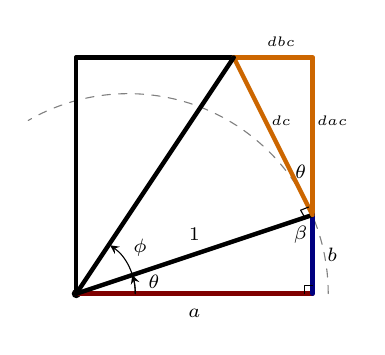
\begin{tikzpicture}[line cap=round]

  \draw [gray,thin,dashed] (3.2,0) arc (0:120:1in); 
  \draw [black,fill=black] (0,0) circle (0.05cm);

  \draw [ultra thick] (0,0) -- (0,3);
  \draw [penColor2,ultra thick] (0,0) -- (3,0);
  \draw [penColor5,ultra thick] (3,1) -- (3,3);
  \draw [penColor,ultra thick] (3,0) -- (3,1);
  \draw [ultra thick] (0,3) -- (2,3);
  \draw [penColor5,ultra thick] (2,3) -- (3,3);

  \draw [ultra thick] (0,0) -- (3,1);
  \draw [penColor5, ultra thick] (3,1) -- (2,3);
  \draw [ultra thick] (0,0) -- (2,3);

  \draw [thin] (2.9,0) -- (2.9,0.1);
  \draw [thin] (2.9,0.1) -- (3,0.1);

  \draw [thin] (2.9,0.97) -- (2.85,1.06);
  \draw [thin] (2.85,1.06) -- (2.95,1.10);




  \draw [->] (.75,0) arc(0:18.4:.75); 
  \draw [rotate=9] (1,0) node {\scriptsize{$\theta$}};
  \draw [->] (.75,0) arc(0:55:.75); 
  \draw [rotate=36] (1,0) node {\scriptsize{$\phi$}};


  \draw (1.5,-0.25) node {\scriptsize{$a$}};
  \draw (3.25,0.5) node {\scriptsize{$b$}};
  \draw (1.5,0.75) node {\scriptsize{$1$}};

  \draw (2.6,2.2) node {\tiny{$\tfrac{d}{c}$}};


  \draw (2.85,1.55) node {\scriptsize{$\theta$}};
  \draw (2.85,0.75) node {\scriptsize{$\beta$}};


  \draw (3.25,2.2) node {\tiny{$\tfrac{da}{c}$}};
  \draw (2.6,3.2) node {\tiny{$\tfrac{db}{c}$}};



    \end{tikzpicture}
  \end{image}






We can now deduce the lengths of the other two pieces of the rectangle in terms of $a$, $b$, $c$, and $d$.










\begin{image}[3in]
    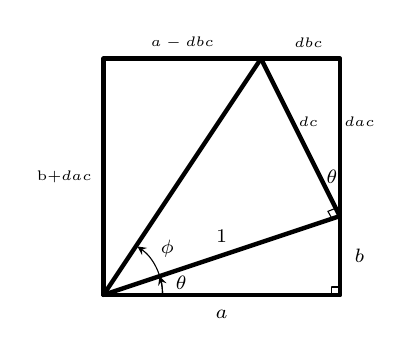
\begin{tikzpicture}[line cap=round]

  \draw [ultra thick] (0,0) -- (0,3);
  \draw [ultra thick] (0,0) -- (3,0);
  \draw [ultra thick] (3,0) -- (3,3);
  \draw [ultra thick] (0,3) -- (3,3);

  \draw [ultra thick] (0,0) -- (3,1);
  \draw [ultra thick] (3,1) -- (2,3);
  \draw [ultra thick] (0,0) -- (2,3);

  \draw [thin] (2.9,0) -- (2.9,0.1);
  \draw [thin] (2.9,0.1) -- (3,0.1);

  \draw [thin] (2.9,0.97) -- (2.85,1.06);
  \draw [thin] (2.85,1.06) -- (2.95,1.10);




  \draw [->] (.75,0) arc(0:18.4:.75); 
  \draw [rotate=9] (1,0) node {\scriptsize{$\theta$}};
  \draw [->] (.75,0) arc(0:55:.75); 
  \draw [rotate=36] (1,0) node {\scriptsize{$\phi$}};


  \draw (1.5,-0.25) node {\scriptsize{$a$}};
  \draw (3.25,0.5) node {\scriptsize{$b$}};
  \draw (1.5,0.75) node {\scriptsize{$1$}};


  \draw (2.9,1.5) node {\scriptsize{$\theta$}};
  \draw (2.6,2.2) node {\tiny{$\tfrac{d}{c}$}};

  \draw (3.25,2.2) node {\tiny{$\tfrac{da}{c}$}};
  \draw (2.6,3.2) node {\tiny{$\tfrac{db}{c}$}};

  \draw (-0.5,1.5) node {\tiny{b+$\tfrac{da}{c}$}};
  \draw (1,3.2) node {\tiny{$a-\tfrac{db}{c}$}};






    \end{tikzpicture}
  \end{image}


We almost have every aspect of this diagram figured out.  We have two angles left.






Let's turn our attention to the right triangle formed in the upper-left corner of the rectangle.

The bottom exterior angle is the sum of $\theta$ and $\phi$.  It is just our two original angles glued together.






\begin{image}[3in]
    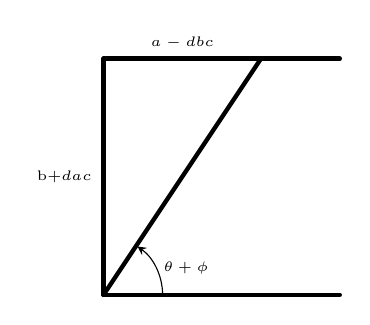
\begin{tikzpicture}[line cap=round]

  \draw [ultra thick] (0,0) -- (0,3);
  \draw [ultra thick] (0,0) -- (3,0);
  \draw [ultra thick] (0,3) -- (3,3);



  
  \draw [ultra thick] (0,0) -- (2,3);

 





  \draw [->] (.75,0) arc(0:55:.75); 
  \draw [rotate=18] (1.1,0) node {\tiny{$\theta + \phi$}};
  %\draw (1.25,2.75) node {\tiny{$\theta + \phi$}};




  \draw (-0.5,1.5) node {\tiny{b+$\tfrac{da}{c}$}};
  \draw (1,3.2) node {\tiny{$a-\tfrac{db}{c}$}};






    \end{tikzpicture}
  \end{image}



If we view the slanted line as the diagonal of a rectangle, then we can see that the upper angle must also measure $\theta + \phi$.










\begin{image}[3in]
    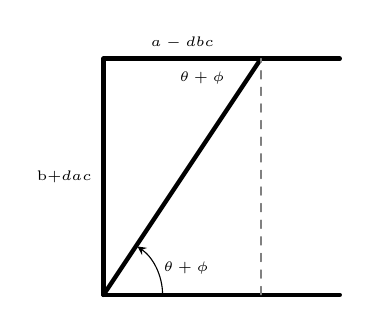
\begin{tikzpicture}[line cap=round]

  \draw [ultra thick] (0,0) -- (0,3);
  \draw [ultra thick] (0,0) -- (3,0);
  \draw [ultra thick] (0,3) -- (3,3);



  
  \draw [ultra thick] (0,0) -- (2,3);

 
  \draw [gray,dashed] (2,0) -- (2,3);




  \draw [->] (.75,0) arc(0:55:.75); 
  \draw [rotate=18] (1.1,0) node {\tiny{$\theta + \phi$}};
  \draw (1.25,2.75) node {\tiny{$\theta + \phi$}};




  \draw (-0.5,1.5) node {\tiny{b+$\tfrac{da}{c}$}};
  \draw (1,3.2) node {\tiny{$a-\tfrac{db}{c}$}};






    \end{tikzpicture}
  \end{image}














Finally, let's resize this triangle by a factor of $c$.









\begin{image}[3in]
    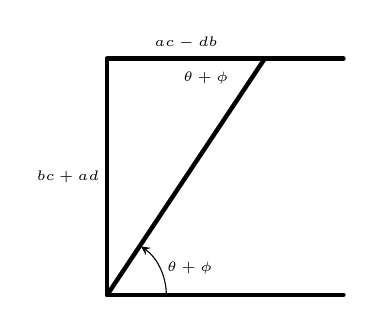
\begin{tikzpicture}[line cap=round]

  \draw [ultra thick] (0,0) -- (0,3);
  \draw [ultra thick] (0,0) -- (3,0);
  \draw [ultra thick] (0,3) -- (3,3);



  
  \draw [ultra thick] (0,0) -- (2,3);

 





  \draw [->] (.75,0) arc(0:55:.75); 
  \draw [rotate=18] (1.1,0) node {\tiny{$\theta + \phi$}};
  \draw (1.25,2.75) node {\tiny{$\theta + \phi$}};




  \draw (-0.5,1.5) node {\tiny{$bc+ad$}};
  \draw (1,3.2) node {\tiny{$ac-db$}};






    \end{tikzpicture}
  \end{image}

These two lengths are familiar. \\



It is upsidedown, but this is the right triangle defined on the unit circle by the product of our two complex numbers:

\[  (a + b \, i) \cdot (c + d \, i) = (ac-bd) + (ad+bc) \, i    \]




Let's flip it over.










\begin{image}[3in]
    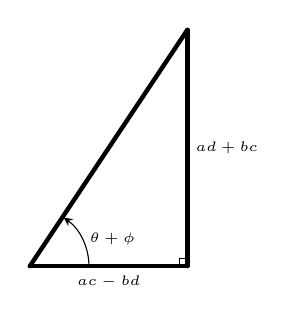
\begin{tikzpicture}[line cap=round]

  \draw [ultra thick] (0,0) -- (2,3);
  \draw [ultra thick] (0,0) -- (2,0);
  \draw [ultra thick] (2,0) -- (2,3);


  \draw [thin] (1.9,0) -- (1.9,0.1);
  \draw [thin] (1.9,0.1) -- (2,0.1);


  \draw [->] (.75,0) arc(0:55:.75); 
  \draw [rotate=18] (1.1,0) node {\tiny{$\theta + \phi$}};





  \draw (2.5,1.5) node {\tiny{$ad+bc$}};
  \draw (1,-0.2) node {\tiny{$ac-bd$}};






    \end{tikzpicture}
  \end{image}









 

\textcolor{red!80!black}{$\blacktriangleright$} When multiplying complex numbers on the unit circle, just add their angles. \\




The product of two complex numbers on the unit circle is again on the unit circle. Its location is given by adding the angles of the two factors.


We can now extend this to all complex numbers by bringing back in their distance from the origin - the modulus. \\




\textcolor{red!80!black}{$\blacktriangleright$} When multiplying any two complex numbers, multiply their moduli and add their angles.



\begin{theorem}  \textbf{\textcolor{green!50!black}{Complex Multiplication (Polar)}}

\[  (r_1, \theta_1) \cdot (r_2, \theta_2) = (r_1 \cdot r_2, \theta_1 + \theta_2)              \]


\end{theorem}




\begin{example}  Squaring \\


The two complex numbers could be the same number. $\frac{1}{\sqrt{2}} + \frac{1}{\sqrt{2}} \, i = \left(1, \frac{\pi}{4} \right)$


\[
\left( \frac{1}{\sqrt{2}} + \frac{1}{\sqrt{2}} \, i \right)^2 = \left(1, \frac{\pi}{4} \right) \cdot \left(1, \frac{\pi}{4} \right)
\]

\[
= \left(1, \frac{\pi}{4} + \frac{\pi}{4} \right) = \left( 1, \frac{\pi}{2} \right) = i
\]




$\frac{1}{\sqrt{2}} + \frac{1}{\sqrt{2}} \, i$ is a square root of $i$.


\end{example}







\begin{example}  Fourth Root \\


We can work the angles backwards as well.  \\

To get a fourth root of $-1$, we would need an angle such that $4$ times the angle is $\pi$.    \\

$\frac{\pi}{4}$ will work.  We need the complex number on the unit circle at an angle of $\frac{\pi}{4}$.  That is $\frac{1}{\sqrt{2}} + \frac{1}{\sqrt{2}} \, i$.


\end{example}













\begin{center}
\textbf{\textcolor{green!50!black}{ooooo-=-=-=-ooOoo-=-=-=-ooooo}} \\

more examples can be found by following this link\\ \link[More Examples of The Unit Circle]{https://ximera.osu.edu/csccmathematics/precalculus2/precalculus2/theUnitCircle/examples/exampleList}

\end{center}







\end{document}
